%!TEX root =机械设计.tex
\chapter{齿轮传动}
\section{齿轮传动的特点}
\begin{paracol}{2}
优点：
\begin{itemize}
\item 传动效率高;
\item 传动比准确;
\item 结构紧凑,承载能力高;
\item 工作可靠,寿命长;
\end{itemize}
\switchcolumn
缺点：
\begin{itemize}
    \item 对齿轮制造、安装要求高;
    \item 齿轮制造需用专用机床及刀具;
    \item 齿轮传动成本及费用高;
    \item 不适宜中心距过大的动力传递;
\end{itemize}

\end{paracol}

\section{齿轮传动的失效形式}
对于齿轮传动的失效形式，需要清楚失效的原因、失效的常见位置还有怎么预防失效。
\subsection{轮齿折断}
轮齿折断\textit{（Teeth breaking-off）}为\textbf{闭式硬齿面齿轮}的主要失效形式。

一般分为弯曲疲劳折断和过载折断两种形式。

力作用使齿根处产生最大拉应力，导致齿轮折断。

于是对于折断部位我们可以看到，对于直齿轮折断一般发生在齿根部位，对于斜齿轮则为局部折断。（斜齿轮接触线倾斜，啮合逐渐进入退出，加上轴向力和偏载，载荷沿齿宽分布不均，端部或局部齿根应力最大，所以常表现为局部折断。）

提高轮齿抗折断的能力:
\begin{enumerate}
    \item 减小齿根应力集中(如增大齿根过渡圆角半径)
    \item 提高安装精度及支承刚度,避免偏载
    \item 改善热处理使其有足够的齿芯韧性和齿面硬度
    \item 齿根部分进行表面强化处理(喷丸、滚压等)
\end{enumerate}

\subsection{齿面疲劳点蚀}
\textbf{齿面疲劳点蚀}是\textbf{闭式软齿面齿轮}的主要失效形式。

疲劳点蚀一般发生在节线附近。

节线附近通常为单齿对啮合,接触应力较大。且节线处相对滑动速度低,不易形成润滑油膜。

\begin{figure}[htbp]
    \centering
    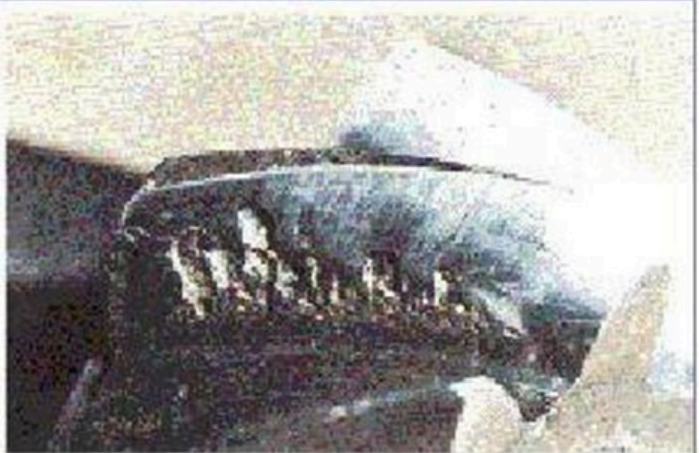
\includegraphics[width=0.8\textwidth]{Figure/齿面疲劳点蚀.png}
    \caption{疲劳点蚀}
    \label{fig:齿面疲劳点蚀}
\end{figure}
防止轮齿疲劳点蚀的措施：
\begin{enumerate}
    \item 提高齿面硬度
    \item 降低表面粗糙度
    \item 采用变位齿轮以增加综合曲率半径
    \item 选用较高粘度润滑油
    \item 提高加工安装精度,改善散热
\end{enumerate}

\subsection{齿面磨损}
开式齿轮的主要失效形式是齿面磨损。
防止齿面磨损措施:
\begin{enumerate}
    \item 提高齿面硬度(我比沙子硬就行)
    \item 降低表面粗糙度
    \item 降低滑动系数
    \item 润滑油清洁更换
    \item 变开式为闭式（我加个罩子就成了吧）
\end{enumerate}

\subsection{齿面胶合}
高速重载齿轮的主要失效形式是齿面胶合。

高速重载下，压力大，滑动速度高，摩擦热就大，产生高温，导致啮合齿面黏结，然后黏结的地方被剪切，导致齿轮失效。

而胶合形式又分为热胶合和冷胶合。

热胶合成因如上，冷胶合一般发生在低速重载，但是缺少润滑油，也会产生冷焊结点。
\begin{figure}[htbp]
    \centering
    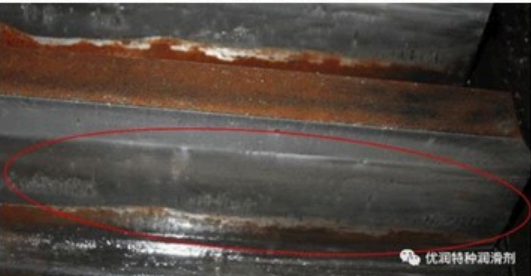
\includegraphics[width=0.8\textwidth]{Figure/齿面胶合.png}
    \caption{齿面胶合}
    \label{fig:齿面胶合}
\end{figure}
防止齿面胶合措施:
\begin{enumerate}
    \item 采用抗胶合能力强的润滑油
    \item 降低滑动速度(变位或减小模数和齿高)
    \item 提高齿面硬度
    \item 降低粗糙度
    \item 配对齿轮有适当的硬度差
    \item 改善润滑与散热条件
\end{enumerate}

\subsection{齿面塑性变形}
低速重载齿轮的主要失效形式是齿面塑性变形。

齿面在过大的摩擦力作用下处于屈服状态,产生沿摩擦力方向的齿面材料的塑性流动,使齿面正确轮廓曲线被破坏。

防止塑性变形措施:
\begin{enumerate}
    \item 采用高粘度的润滑油或加极压添加剂。
    \item 提高齿面硬度
\end{enumerate}

\section{设计准则}
\begin{figure}[htbp]
    \centering
    \resizebox{\textwidth}{!}{% 齿轮传动设计准则流程图
\begin{tikzpicture}[
    node distance=1.2cm and 1.5cm,
    >=latex,
    box/.style={
        rectangle,
        draw,
        fill=#1,
        minimum height=0.8cm,
        minimum width=3.2cm,
        align=center,
        font=\small\bfseries
    },
    box/.default=blue!20,
    graybox/.style={
        rectangle,
        draw,
        fill=gray!40,
        minimum height=0.7cm,
        minimum width=3cm,
        align=center,
        font=\small
    },
    greenbox/.style={
        rectangle,
        draw,
        fill=green!15,
        minimum height=0.7cm,
        minimum width=3.5cm,
        align=center,
        font=\small
    },
    arrow/.style={
        ->,
        thick,
        >=latex
    }
]

% 顶部节点
\node[box] (top) {闭式齿轮传动};

% 第二层节点
\node[box, below left=1.2cm and 1.5cm of top] (soft) {软齿面齿轮\\(HBS$\leqslant$350)};
\node[box, below right=1.2cm and 1.5cm of top] (hard) {硬齿面齿轮\\(HBS$>$350)};

% 第三层节点
\node[graybox, below=of soft] (soft_fail) {齿面疲劳点蚀};
\node[graybox, below=of hard] (hard_fail) {齿根弯曲疲劳折断};

% 第四层节点
\node[greenbox, below=of soft_fail] (soft_rule) {齿面接触疲劳强度准则};
\node[greenbox, below=of hard_fail] (hard_rule) {齿根弯曲疲劳强度准则};

% 开式齿轮传动
\node[box, below left=1.2cm and 2cm of soft_rule] (open) {开式齿轮传动};
\node[graybox, right=of open] (open_fail) {齿面磨损};
\node[greenbox, below right=0.8cm and 0.5cm of open_fail] (open_rule) {增大m和降低许用弯曲应力};

% 连接线
\draw[arrow] (top) -- (soft);
\draw[arrow] (top) -- (hard);
\draw[arrow] (soft) -- (soft_fail);
\draw[arrow] (hard) -- (hard_fail);
\draw[arrow] (soft_fail) -- (soft_rule);
\draw[arrow] (hard_fail) -- (hard_rule);
\draw[arrow] (open) -- (open_fail);
\draw[arrow] (open_fail) -- (open_rule);
\draw[arrow] (open_fail) -- (hard_rule);

\end{tikzpicture}
}
    \caption{齿轮传动设计准则}
    \label{fig:齿轮传动设计准则}
\end{figure}

\section{齿轮传动的计算载荷}
\begin{formula}
    \begin{equation}
        F_{nc}=KF_{n}
    \end{equation}
其中：
\begin{itemize}
    \item $F_{nc}$：计算法向载荷
    \item $K$：载荷系数
    \item $F_{n}$：名义法向载荷
\end{itemize}
\end{formula}
对于载荷系数$K$，有
\begin{equation}
    K=K_{A}K_{v}K_{\beta}K_{\alpha}
\end{equation}

下面逐一看看这四个系数。

\subsection{工作情况系数$K_{A}$}
考虑齿轮啮合时,外部因素引起的附加动载荷对传动的影响。

外部因素:与原动机、工作机、联轴器等有关。
\subsection{动载荷系数$K_{v}$}
考虑齿轮制造、安装误差及弹性变形等内部因素引起的附加动载荷的影响。

\subsection{齿向载荷分布系数$K_{\beta}$}
考虑轴的弯曲、扭转变形、轴承、支座弹性变形及制造和装配误差而引起的沿齿宽方向载荷分布不均匀的影响。

影响因素：
\begin{enumerate}
    \item \textbf{支承情况}：对称布置——好；非对称布置——差；悬臂布置——差；
    \item \textbf{齿轮宽度}：齿轮宽度越大，齿向载荷分布系数越大；
    \item \textbf{齿面硬度}：齿面硬度越高，越易偏载，齿面较软时有变形退让；
    \item \textbf{制造、安装精度}：精度越高，齿向载荷分布系数越小。
\end{enumerate}

减小 $K_{\beta}$ 的措施：
\begin{enumerate}
    \item 提高制造安装精度；
    \item 提高支承刚度，尽量避免悬臂布置；
    \item 采用鼓形齿（drum tooth），齿向鼓形量取 $(0.0005\sim0.001)b$；
    \item 螺旋角修形（helical angle correction）——沿小齿轮齿宽进行修形，以补偿由于轴的弯曲和扭转变形引起的啮合线位置的改变。
\end{enumerate}

\subsection{齿间载荷分配系数$K_{\alpha}$}
考虑同时有多对齿啮合时,各对轮齿间载荷分配不均匀的影响。

\section{直齿圆柱齿轮传动的强度计算}
\subsection{受力分析}
\begin{figure}[htbp]
    \centering
    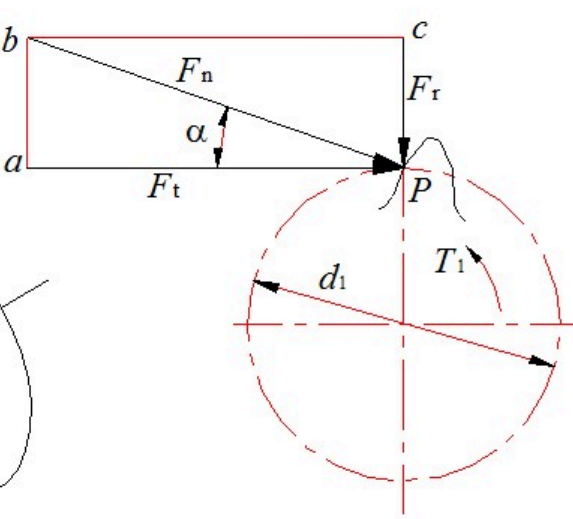
\includegraphics[width=0.5\textwidth]{Figure/轮齿受力分析.png}
    \caption{轮齿受力分析}
    \label{fig:轮齿受力分析}
\end{figure}
如上图所示，法向力$F_{n}$可以正交分解为径向力$F_{r}$和切向力$F_{t}$，且方向遵循“主反从同”。

\subsection{齿根弯曲疲劳强度计算}
计算假设：
\begin{enumerate}
    \item 单对齿啮合。
    \item 载荷作用于齿顶。
    \item 按悬臂梁计算。
    \item 只考虑弯曲应力。
    \item 用重合度系数考虑非单对齿啮合。
    \item 危险截面用$30^\circ$切线法。
\end{enumerate}
\begin{formula}
    \begin{equation}
        \sigma_{F}=\frac{2 K T_{1}}{b d_{1} m} \cdot Y_{F a} Y_{S a} Y_{\varepsilon}
    \end{equation}
其中：
\begin{itemize}
    \item $\sigma_{F}$：齿根弯曲应力（MPa）
    \item $K$：载荷系数
    \item $T_{1}$：小齿轮传递的转矩（N·mm）
    \item $b$：齿宽（mm）
    \item $d_{1}$：小齿轮分度圆直径（mm）
    \item $m$：模数（mm）
    \item $Y_{Fa}$：齿形系数（考虑齿形对齿根弯曲应力的影响）
    \item $Y_{Sa}$：应力修正系数（考虑齿根过渡圆角处应力集中的影响）
    \item $Y_{\varepsilon}$：重合度系数（考虑重合度对齿根弯曲应力的影响）
\end{itemize}
\end{formula}

引入齿宽系数$\Phi_d=\frac{b}{d_{1}}$，则有
\begin{formula} [校核公式]
    \begin{equation}
        \sigma_{F}=\frac{2 K T_{1} Y_{F a} Y_{s a} Y_{\varepsilon}}{\phi_{d} m^{3} Z_{1}^{2}} \leq[\sigma]_{F}
    \end{equation}
\end{formula}
\begin{formula} [设计公式]
    \begin{equation}
        m \geq \sqrt[3]{\frac{2 K T_{1}}{\phi_{d} Z_{1}^{2}} \cdot \frac{Y_{F a} Y_{s a} Y_{\varepsilon}}{[\sigma]_{F}}}
    \end{equation}
\end{formula}

\section{齿面接触疲劳强度计算}
设计依据:两圆柱体接触赫兹公式
\begin{formula}[接触疲劳强度的校核公式]
    \begin{equation}
        \sigma_{H}=Z_{E} \cdot Z_{\varepsilon} \cdot Z_{H} \sqrt{\frac{K F_{t}}{b d_{1}} \cdot \frac{u \pm 1}{u}} \leq[\sigma]_{H}
    \end{equation}
其中：
\begin{itemize}
    \item $\sigma_{H}$：齿面接触应力（MPa）
    \item $Z_{E}$：弹性影响系数（与两齿轮材料的弹性模量、泊松比有关）
    \item $Z_{H}$：区域系数（考虑节点处齿廓形状对接触应力的影响）
    \item $Z_{\varepsilon}$：重合度系数
    \item $K$：载荷系数
    \item $F_{t}$：圆周力（N），$F_{t}=2T_{1}/d_{1}$
    \item $b$：齿宽（mm）
    \item $d_{1}$：小齿轮分度圆直径（mm）
    \item $u$：齿数比（$u=z_{2}/z_{1}$），外啮合取“$+$”，内啮合取“$-$”
    \item $[\sigma]_{H}$：许用接触应力（MPa）
    \item $T_{1}$：小齿轮传递的转矩（N·mm）
    \item $\phi_{d}$：齿宽系数（$\phi_{d}=b/d_{1}$）
\end{itemize}
\end{formula}

\begin{formula} [设计公式]
    \begin{equation}
        d_{1} \geq \sqrt[3]{\frac{2 K T_{1}}{\phi_{d}} \cdot \frac{u \pm 1}{u}\left(\frac{Z_{H} Z_{E} Z_{\varepsilon}}{[\sigma]_{H}}\right)^{2}}
    \end{equation}
\end{formula}
